Die Nutzung von EC2-Instanzen ist mit einem Zahlungsmodell verbunden. Die Wahl des Zahlungsmodells ist von entscheidender Bedeutung, um den besten Preis für EC2-Instanzen zu erzielen.
%EC2 and RDS(DB) spend are often on of the main portions of your overall AWS Bill t.ly/Mqwn
Die von Amazon Web Services angebotenen Zahlungsmodelle werden im Folgenden dargestellt.
\\\\
Das On-Demand-Modell beinhaltet keine langfristigen Verpflichtungen, es ist daher die teuerste Alternative, die auf Stundenbasis berechnet wird. Die Modelle Saving Plans und Reserved Instances erfordern den Abschluss von Verträgen über ein oder drei Jahre, um günstige Preise zu erhalten. EC2-Spot-Instanzen sind das kostengünstigste Modell , haben aber den Nachteil, dass ihre Verfügbarkeit nicht immer garantiert ist.
\\\\
Jedes Zahlungsmodell hat seine Vor- und Nachteile und eignet sich für unterschiedliche Anwendungsfälle. Gute Ergebnisse können auch durch die Kombination mehrerer Zahlungsmodelle erzielt werden[SAG DER CLOUD-EXPERT/FIRMA]. Dies wird in Unterkapitel \ref{sssec:num2.4} behandelt.[WIRD ES?]
\\\\
In dieser Arbeit wird nicht darauf eingegangen, wie die richtige Server-Instanz ausgewählt werden sollte, da die Auswahl von individuellen Anforderungen abhängt, die von Fall zu Fall unterschiedlich sind. 

Im Allgemeinen wird empfohlen Instanzen so nahe wie möglich an den Ressourcen\footnote{Mit Ressourcen sind Cloud-Dienste gemeint}[ERKLÄRUNG NÖTIG?], mit denen sie kommunizieren werden, zu platzieren. 
Die beste Leistung wird außerdem angestrebt, indem sich diese Instanzen in räumlicher Nähe zur Mehrzahl der Endnutzer, befinden. 

%Vor- und Nachteile noch tabellarisch aufzulisten??
%https://youtu.be/Q5wSvUVPyYY?t=678

%Excess capacity/Spot Instances
\subsection{On-Demand / Nutzungsabhängige Zahlung}
Bei diesem Zahlungsmodell besteht keine Notwendigkeit, ein festes Anfangsbudget festzulegen. Die Kosten richten sich nach dem Verbrauch auf der Grundlage der Nutzungsstunden.
\\
Dieses Modell eignet sich für Projekte, bei denen nicht viel vorhersehbar ist und die Möglichkeit besteht, dass das Projekt in kurzer Zeit abgeschlossen sein wird, so dass es keinen Sinn macht, eine langfristige Verpflichtung einzugehen.
\\
Hier einige Beispiele von EC2-Instanzen im On-Demand Zahlungsmodell.
\begin{figure}
    \centering
    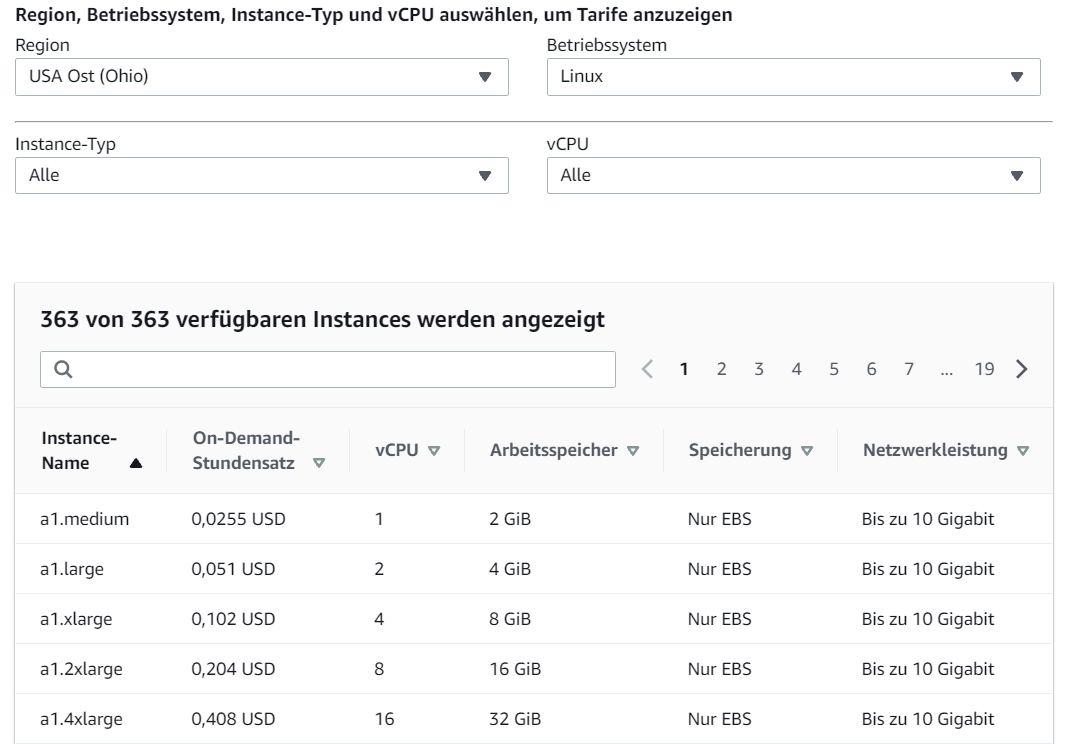
\includegraphics[scale=0.4]{sources/On-Demand-Pläne für Amazon EC2}\label{fig:OnDemand_Preise}\\
    \caption[On-Demand Preise für Amazon EC2]{}
    \label{fig:OnDemand_Preise}  On-Demand Preise für Amazon EC2 {\cite{AMZ02}}
  \end{figure}

  WARUM IST DIESE ABB.?

Der Preis für dieses Modell variiert je nach Instanz Typ, Region und der übertragenen Datenmenge. 
Die aktuellen Preise für die verschiedenen Regionen sind auf der Amazon-Website in der Sektion EC2 - On-Demand-Preise\footnote{https://aws.amazon.com/de/ec2/pricing/on-demand/} zu finden.
In der \autoref{fig:OnDemand_Preise} werden die für die Region Ohio verfügbaren Linux-Instanzen gezeigt. Es ist zu beachten, dass Instanzen mit denselben Eigenschaften, aber in verschiedenen Regionen, unterschiedliche Preise haben können.

\subsection{Reservierte Instanzen und Saving Plans}
%t.ly/JUWq
%https://www.youtube.com/watch?v=c_zlPQimrvY
\begin{flushleft}
    Die Zahlungsmodelle Reservierte Instanzen und Saving Plans sind sich sehr ähnlich. Beide kommen mit einer gleichbleibenden  Nutzungsverpflichtung, die in €/Stunden gemessen wird.

    Um die reduzierten Preise  zu bekommen, müssen Verträge 1 oder 3 Jahre abgeschlossen werden.

    Nachfolgend werden die prozentualen Einsparungen gemäß des jeweiligen Modells gezeigt.
\end{flushleft}

\begin{table}[h!]
    \centering
    \begin{tabular}{ |p{3cm}||p{3cm}|p{3.6cm}|p{3.6cm}|  }
        \hline
        \multicolumn{4}{|c|}{Einsparungen nach Modell}                                                                    \\
        \hline
        Compute Savings Plans & EC2-Instance Savings Plans & Convertible Reserved Instances & Standard Reserved Instances \\
        \hline
        bis zu 66\%           & bis zu 72\%
                              & bis zu 54\%)               & bis zu 72\%
        \\
        \hline
    \end{tabular}
    {\cite{AMZ07,AMZ11}}
\end{table}
Die ersten beiden Optionen in der obigen Tabelle, die Saving Plans, unterscheiden sich dadurch, dass die Compute Savings Plans die Flexibilität bieten, EC2-Instanzen nach Familie\footnote{\cite{AWS1}, Seite 95}, Größe, Availability Zone (AZ), Betriebssystem oder Mandant zu wechseln.
\begin{quote}
    „Bei Compute Savings Plans können Sie beispielsweise jederzeit von C4- auf M5-Instances wechseln, eine Workload von EU (Irland) nach EU (London) verlagern oder eine Workload von EC2 auf Fargate oder Lambda verschieben. Dabei zahlen Sie automatisch weiterhin den Savings Plans-Preis.”
    {\cite{AMZ11}}
\end{quote}

Bei den EC2-Instance Saving Plans hingegen muss eine Instance-Familie in einer bestimmten Region ausgewählt werden.  Dies reduziert automatisch die Kosten für die ausgewählte Instanz-Familie in der jeweiligen Region, unabhängig von Availability Zone, Größe, Betriebssystem oder Mandant.
\\
Die Festlegung eines festen Stundensatzes über einen langen Zeitraum bietet die Möglichkeit, künftige Kosten zu planen[ZITAT/BASIERT AUF...]
\\
%Folgenden Kriterien definieren den Preis von EC2-Instanzen bei Saving Plans:
%Vertraglaufzeit, Vorabzahlung, Betriebssystem,Region, Mandant
AUCH FÜR RIs?
%3 Arten von S. Plans: Compute and EC2 Instance
\subsubsection{Vorauszahlung}
Zusätzlich gibt es bei Saving Plans und reservierten Instanzen die Option im Voraus zu zahlen.
Im Gegenzug wird ein niedrigerer Preis angeboten.

Amazon bietet drei verschiedene Optionen an. Diese sind teilweise, keine oder vollständige Vorauszahlung.

Bei teilweiser Vorauszahlung ist eine Anzahlung von etwa 50\% zu leisten.

(To-Do: wie viel kann in den verschiedenen Szenarien eingespart werden).

\subsection{Spot Instanzen }
EC2 Spot-Instances bieten die Möglichkeit aus von anderen Nutzern ungenutzter EC2-Instances zu profitieren.
Mit einem Preisvorteil von bis zu 90 \% gegenüber normalen On-Demand-Instanzen sind Spot-Instanzen ideal für fehlertolerante Anwendungen wie auf Containern ausgeführte Workloads, CI/CD, Bigdata-Anwendungen und ähnliches.
\\
\subsubsection{Unterbrechbarkeit}
Es ist zu beachten, dass Spot-Instanzen jederzeit unterbrochen werden können.   

Einer der Gründe ist die Preisüberschreitung[RICHTIG?] der Instanz. Wenn Spot-Instanzen angefordert werden, wird einen Maximalpreis festgelegt. Sollte der Preis der Instanz höher als das eingegebener Maximalpreis, wird die Instanz für die aktuelle Einstellung nicht mehr verfügbar sein.

Ein anderes Szenario ist, wenn der Instanzanbieter die Instanz erneut anfordert. Falls eine Spot-Instanz unterbrochen wird, benachrichtigt Amazon EC2 2 Minuten im Voraus. Dieses Ereignis ist verfügbar auf CloudWatch und es kann einen Alarm dafür eingestellt werden.
\\
Daher sollten kritische Anwendungen nicht nur mit EC2 Spot-Instanzen laufen.
%Um von der Preisvorteile der Spot-Instanzen zu profitieren und Ausfälle zu vermeiden, sollten in Kombination weitere Zahlungsmodelle verwenden werden.
%\\
%Zum Beispiel eine Kombination aus Spot-Instanzen für die erwarteten Last und On-Demand-Instanzen für die dynamischen Last.
%https://aws.amazon.com/de/ec2/spot/pricing/

%2 OPTIONEN: LOWEST PRICE OR DIVERSIFIED ACROSS n POOLS TO AVOID DOWNS https://www.linkedin.com/learning/aws-automation-and-optimization/request-spot-instances-part-2?autoAdvance=true&autoSkip=true&autoplay=true&resume=false&u=79182202
\subsection{Wahl des Zahlungsmodells} \label{sssec:num2.4}
%Vor- und Nachteile? 
Die folgende Tabelle fasst die Eigenschaften der Zahlungsmodelle für Instanzen zusammen und listet typische Applikationen je nach Zahlungsmodell auf.
Abb. AKTUELL?
\begin{figure}[h!]
    \centering
    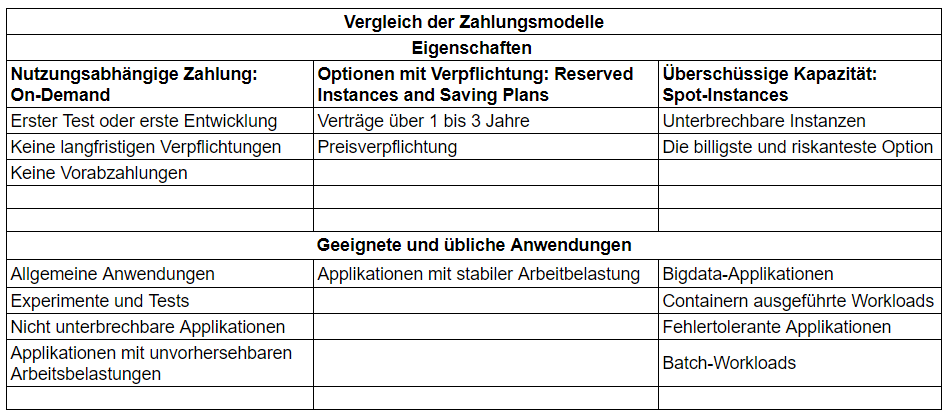
\includegraphics[scale=0.6]{sources/Vergleich_der_Zahlungsmodelle}\label{fig:Vergleich_der_Zahlungsmodelle}\\
    \caption[Vergleich der Zahlungsmodelle]{}
    \label{fig:Vergleich_der_Zahlungsmodelle}  Vergleich der Zahlungsmodelle \\
    Quelle: Eigene Darstellung.
  \end{figure}

%To read planned at 21.11:
%https://www.pcapps.com/services/aws-reserved-vs-on-demand-instances/
%https://jaychapel.medium.com/aws-reserved-instances-versus-on-demand-which-is-better-e7f77f1f9582
%https://www.cloudhealthtech.com/blog/aws-reserved-instances-vs-on-demand#:~:text=In%20terms%20of%20compute%20options,of%20an%20On%20Demand%20instance.

%https://youtu.be/mKEdhmJ2udA?t=79
%Automate the selection to get the best price
%https://spot.io/aws-cost-optimization-calculator/
\textbf{Summary/Fazit}
\\\\
In diesem Kapitel wurden die verschiedenen Zahlungsmodelle für EC2-Instanzen untersucht. Es wurden Hinweise für die Auswahl des richtigen Zahlungsmodells in verschiedenen Szenarien gegeben. Dies wurde erklärt, um die Preisvorteile[RICHTIG?] von den Zahlungsmodellen zu nutzen. 
%En el capitulo monitoreo de costes  se mostrarán herramientas como X(CloudWatch) con las que podremos verificar si la desicion realizada fue la correcta. Para el modelo de pago On-Demand no hay ninguna redccion de los costos, pero existen medidas para aun asi reducir el uso de las instancias. Dichas medidas seran profundizadas en capitulo medidas de optimizacion
Im Kapitel Kostenüberwachung wird X(CloudWatch?) vorgestellt, mit dem überprüft werden kann, ob das ausgewählte Zahlungsmodell tatsächlich das Richtige für den betreffenden Anwendungsfall ist. Für das On-Demand-Zahlungsmodell gibt es keine Kostenreduzierung, aber es gibt Maßnahmen, um die Nutzung von Instanzen zu reduzieren. Auf diese Maßnahmen wird im Kapitel über Optimierungsmaßnahmen näher eingegangen.